\iffalse
\let\negmedspace\undefined
\let\negthickspace\undefined
\documentclass[journal,12pt,twocolumn]{IEEEtran}
\usepackage{cite}
\usepackage{circuitikz}
\usepackage{amsmath,amssymb,amsfonts,amsthm}
\usepackage{algorithmic}
\usepackage{graphicx}
\usepackage{textcomp}
\usepackage{xcolor}
\usepackage{txfonts}
\usepackage{listings}
\usepackage{enumitem}
\usepackage{mathtools}
\usepackage{gensymb}
\usepackage{comment}
\usepackage[breaklinks=true]{hyperref}
\usepackage{tkz-euclide} 
\usepackage{listings}
\usepackage{gvv}                                        
\def\inputGnumericTable{}                                 
\usepackage[latin1]{inputenc}                                
\usepackage{color}                                            
\newtheorem{theorem}{Theorem}[section]
\usepackage{array}                                            
\usepackage{longtable}                                       
\usepackage{calc}                                             
\usepackage{multirow}                                         
\usepackage{hhline}                                           
\usepackage{ifthen}                                           
\usepackage{lscape}
\newtheorem{problem}{Problem}
\newtheorem{proposition}{Proposition}[section]
\newtheorem{lemma}{Lemma}[section]
\newtheorem{corollary}[theorem]{Corollary}
\newtheorem{example}{Example}[section]
\newtheorem{definition}[problem]{Definition}
\newcommand{\BEQA}{\begin{eqnarray}}
\newcommand{\EEQA}{\end{eqnarray}}
\newcommand{\define}{\stackrel{\triangle}{=}}
\theoremstyle{remark}
\newtheorem{rem}{Remark}
\begin{document}
\bibliographystyle{IEEEtran}
\vspace{3cm}
\title{GATE 22 IN/33}
\author{EE23BTECH11040 - Manoj Kumar Ambatipudi$^{*}$% <-this % stops a space
}
\maketitle
\newpage
\bigskip
\renewcommand{\thefigure}{\theenumi}
\renewcommand{\thetable}{\theenumi}
\textbf{QUESTION:}
In the bandpass filter circuit shown, $R_0 = 50\Omega$, $L_0 = 1 mH$, $C_0 = 10nF$. The q factor of the filter is 
\begin{figure}[h]
\renewcommand\thefigure{1}
    \centering
    \begin{circuitikz}[american]
    \draw (0,0) to [L=$L_0$, *-] (2,0) to [C=$C_0$] (4,0) to [R=$R_0$] (4,-2) to [short, -*] (0,-2);
    \draw (4,-0.3) to[short, -*] (6,-0.3);
    \draw (4,-1.7) to[short, -*] (6,-1.7);

    \node at (6,-1) {Output};
    \node at (0,-1) {Input};
    \end{circuitikz}
\end{figure}


\textbf{SOLUTION:}
\fi
\begin{table}[h]
\renewcommand\thetable{1}
    \centering
    \begin{tabular}{|c|c|c|}
    \hline
     Variable & Description&Value\\\hline
        $R_0$ & Resistance & $50\Omega$ \\\hline
        $L_0$ & Inductance & $1mH$ \\\hline
        $C_0$ & Capacitance & $10nF$\\\hline
        $\omega_0$& Resonant Angular Frequency & $\frac{1}{\sqrt{L_0C_0}}$\\\hline
    \end{tabular}
    \caption{Variables and their description}
    \label{tab_22_33_1}
\end{table}
\\
The corresponding Laplace domain circuit is 
\begin{figure}[h]
\renewcommand\thefigure{2}
    \centering
    \begin{circuitikz}[american]
    \draw (0,0) to [generic=$sL_0$, *-] (2,0) to [generic=$\frac{1}{sC_0}$] (4,0) to [generic=$R_0$] (4,-2) to [short, -*] (0,-2);
    \draw (4,-0.3) to[short, -*] (6,-0.3);
    \draw (4,-1.7) to[short, -*] (6,-1.7);
    \node at (6,-1) {Output};
    \node at (0,-1) {Input};
    \end{circuitikz}
\end{figure}


Input $X\brak{s}$ can be written as
\begin{align}
    X\brak{s} = I\brak{s}\brak{sL_0 + \frac{1}{sC_0} + R_0} 
\end{align}
Output $Y\brak{s}$ can be written as 
\begin{align}
    Y\brak{s} = I\brak{s}R_0
\end{align}
Transfer function $H\brak{s}$ can be written as 
\begin{align}
    H\brak{s} &= \frac{Y\brak{s}}{X\brak{s}}\\ &= \frac{sC_0R_0}{s^2C_0L_0 + C_0R_0s + 1}
\end{align}
substituting $s = j\omega$
\begin{align}
    H\brak{j,\omega} = \frac{j\omega C_0R_0}{-\omega^2C_0L_0 + jC_0R_0\omega + 1}\\
\implies \abs{H\brak{j,\omega}} = \frac{\omega C_0R_0}{\sqrt{\brak{1-\omega^2C_0L_0}^2 + \brak{C_0R_0\omega}^{2}}}
\end{align}
Differentiating w.r.t $\omega$ and equating to 0, we get 
\begin{align}
    \frac{d\abs{H\brak{j,\omega}}}{d\omega} &= \frac{C_0R_0}{\sqrt{\brak{1-\omega^2C_0L_0}^2 + \brak{C_0R_0\omega}^{2}}} +\notag\\& \frac{\omega C_0R_0}{2\brak{\brak{1-\omega^2C_0L_0}^2 + \brak{C_0R_0\omega}^{2}}^{\frac{3}{2}}}\notag\\&\brak{2\omega\brak{C_0R_0}^2-2\brak{1-\omega^2C_0L_0}2\omega} &= 0\\
    \implies \omega_0 &= \frac{1}{\sqrt{L_0C_0}}\label{eq_22_33_1}
\end{align}
from \tabref{tab_22_33_1}, 
\begin{align}
    \omega_0 = 316227.76
\end{align}
$Q-factor$ defined with reference to inductor
\begin{align}
    Q &= \abs{\frac{V_L}{V_R}}_{\omega_0}\\
      &= \frac{L_0\omega_0}{R_0}\\
      &= \frac{1}{R_0}\sqrt{\frac{L_0}{C_0}} \quad\brak{\text{from \eqref{eq_22_33_1}}}
\end{align}
$Q-factor$ defined with reference to capacitor
\begin{align}
    Q &= \abs{\frac{V_C}{V_R}}_{\omega_0}\\
      &= \frac{1}{C_0\omega_0R_0}\\
      &= \frac{1}{R_0}\sqrt{\frac{L_0}{C_0}} \quad\brak{\text{from \eqref{eq_22_33_1}}}
\end{align}
Substituting the values from \tabref{tab_22_33_1}, we get
\begin{align}
    Q = 200
\end{align}
\begin{figure}
\renewcommand\thefigure{1}
    \centering
    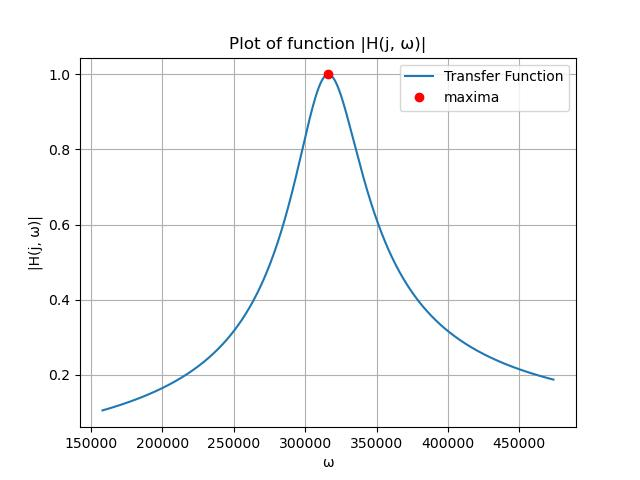
\includegraphics[width=1.0\columnwidth]{2022/IN/33/figs/fig_1.jpg}
    \caption{Transfer function $\abs{H\brak{j, \omega}}$ taken from python3}
    \label{fig:enter-label}
\end{figure}
